% ============================================================================
% GAUSSIAN FILTERS (KALMAN FILTERS) - EXAM NOTES
% Focus: Dynamics model construction, Jacobian computation, EKF
% ============================================================================

\section{Quick Reference: Kalman Filters}

\begin{tcolorbox}[colback=yellow!10!white,colframe=orange!75!black,title=\textbf{Kalman Filter Family - Fast Reference}]

\textbf{Common Structure:} All represent belief as Gaussian $\mathcal{N}(\mu_t, \Sigma_t)$

\vspace{2mm}
\begin{tabular}{|l|l|l|}
\hline
\textbf{Filter} & \textbf{System} & \textbf{Key Feature} \\
\hline
KF & Linear & Exact, closed-form \\
EKF & Nonlinear & Linearization via Jacobians \\
UKF & Nonlinear & Derivative-free, sigma points \\
\hline
\end{tabular}

\vspace{3mm}
\textbf{Kalman Filter (Linear):}
\begin{align*}
\text{Dynamics: } & x_t = A_t x_{t-1} + B_t u_t + \epsilon_t, \quad \epsilon_t \sim \mathcal{N}(0, R_t) \\
\text{Measurement: } & z_t = C_t x_t + \delta_t, \quad \delta_t \sim \mathcal{N}(0, Q_t)
\end{align*}

\textbf{Extended Kalman Filter (Nonlinear):}
\begin{align*}
\text{Dynamics: } & x_t = g(x_{t-1}, u_t) + \epsilon_t, \quad \epsilon_t \sim \mathcal{N}(0, R_t) \\
\text{Measurement: } & z_t = h(x_t) + \delta_t, \quad \delta_t \sim \mathcal{N}(0, Q_t) \\
\text{Jacobians: } & G_t = \frac{\partial g}{\partial x}\bigg|_{x=\mu_{t-1}}, \quad H_t = \frac{\partial h}{\partial x}\bigg|_{x=\bar{\mu}_t}
\end{align*}

\textbf{Update Equations (both KF and EKF):}
\begin{align*}
\text{Predict: } & \bar{\mu}_t = g(\mu_{t-1}, u_t), \quad \bar{\Sigma}_t = G_t \Sigma_{t-1} G_t^T + R_t \\
\text{Update: } & K_t = \bar{\Sigma}_t H_t^T (H_t \bar{\Sigma}_t H_t^T + Q_t)^{-1} \\
& \mu_t = \bar{\mu}_t + K_t (z_t - h(\bar{\mu}_t)) \\
& \Sigma_t = (I - K_t H_t)\bar{\Sigma}_t
\end{align*}

\end{tcolorbox}

% ============================================================================
\section{Recipe: Building Dynamics Models for EKF}
% ============================================================================

\subsection{Step-by-Step Process for Constructing State-Space Models}

\begin{tcolorbox}[colback=green!5!white,colframe=green!60!black,title=Dynamics Modeling Recipe]

\textbf{Step 1: Choose State Variables}
\begin{itemize}
    \item Select minimum set of variables that completely describe system
    \item Typically: positions, velocities, angles, angular velocities
    \item State vector: $x = [x_1, x_2, \ldots, x_n]^T$
\end{itemize}

\textbf{Step 2: Write Physics Equations}
\begin{itemize}
    \item Apply Newton's laws, Kirchhoff's laws, energy conservation, etc.
    \item Express as differential equations: $\dot{x} = f(x, u)$
\end{itemize}

\textbf{Step 3: Discretize (if continuous)}
\begin{itemize}
    \item Use Euler: $x_{t+1} = x_t + \dot{x}_t \cdot \Delta t$
    \item Or exact solution if available
    \item Result: $x_t = g(x_{t-1}, u_t)$
\end{itemize}

\textbf{Step 4: Define Measurement Model}
\begin{itemize}
    \item What do sensors actually measure?
    \item Express measurements as function of state: $z_t = h(x_t)$
\end{itemize}

\textbf{Step 5: Compute Jacobians}
\begin{itemize}
    \item $G_t = \frac{\partial g}{\partial x}\bigg|_{x=\mu_{t-1}}$ - how dynamics change with state
    \item $H_t = \frac{\partial h}{\partial x}\bigg|_{x=\bar{\mu}_t}$ - how measurements change with state
\end{itemize}

\textbf{Step 6: Specify Noise Covariances}
\begin{itemize}
    \item $R_t$ - process noise (dynamics uncertainty)
    \item $Q_t$ - measurement noise (sensor uncertainty)
\end{itemize}

\end{tcolorbox}

% ============================================================================
\subsection{Jacobian Computation - The Critical Step}
% ============================================================================

\begin{tcolorbox}[colback=red!5!white,colframe=red!75!black,title=\textbf{EXAM CRITICAL: Jacobian Structure}]

For state vector $x = [x_1, x_2, \ldots, x_n]^T$ and dynamics $g = [g_1, g_2, \ldots, g_n]^T$:

\vspace{2mm}
\textbf{Jacobian Matrix Structure:}
\begin{equation}
G_t = \frac{\partial g}{\partial x} =
\begin{bmatrix}
\frac{\partial g_1}{\partial x_1} & \frac{\partial g_1}{\partial x_2} & \cdots & \frac{\partial g_1}{\partial x_n} \\[5pt]
\frac{\partial g_2}{\partial x_1} & \frac{\partial g_2}{\partial x_2} & \cdots & \frac{\partial g_2}{\partial x_n} \\[5pt]
\vdots & \vdots & \ddots & \vdots \\[5pt]
\frac{\partial g_n}{\partial x_1} & \frac{\partial g_n}{\partial x_2} & \cdots & \frac{\partial g_n}{\partial x_n}
\end{bmatrix}
\end{equation}

\textbf{Memory Aid:}
\begin{itemize}
    \item \textbf{Rows} correspond to \textbf{output equations} ($g_1, g_2, \ldots$)
    \item \textbf{Columns} correspond to \textbf{state variables} ($x_1, x_2, \ldots$)
    \item Element $G_{ij}$ = how output $i$ changes with state variable $j$
\end{itemize}

\textbf{Common Derivatives to Remember:}
\begin{align*}
\frac{\partial}{\partial \theta}[\sin\theta] &= \cos\theta, \quad \frac{\partial}{\partial \theta}[\cos\theta] = -\sin\theta \\
\frac{\partial}{\partial x}[ax + b] &= a, \quad \frac{\partial}{\partial x}[x^2] = 2x \\
\frac{\partial}{\partial x}[e^{ax}] &= ae^{ax}, \quad \frac{\partial}{\partial x}[\ln x] = \frac{1}{x}
\end{align*}

\end{tcolorbox}

% ============================================================================
\section{Example: Dynamics Models for Common Systems}
% ============================================================================

\subsection{Example 1: DC Motor}

\begin{tcolorbox}[colback=blue!5!white,colframe=blue!75!black,title=DC Motor Dynamics]

\textbf{System:} DC motor with back-EMF

\textbf{State:} $x = [\theta, \omega, i]^T$ (angle, angular velocity, current)

\textbf{Control:} $u = V$ (applied voltage)

\textbf{Physics Equations:}
\begin{align}
L\frac{di}{dt} &= V - Ri - K_e \omega \quad \text{(Kirchhoff's voltage law)} \\
J\frac{d\omega}{dt} &= K_t i - b\omega - \tau_L \quad \text{(Newton's law)} \\
\frac{d\theta}{dt} &= \omega \quad \text{(kinematics)}
\end{align}

where: $L$ = inductance, $R$ = resistance, $K_e$ = back-EMF constant, $K_t$ = torque constant, $J$ = inertia, $b$ = damping, $\tau_L$ = load torque

\textbf{Continuous Dynamics:}
\begin{equation}
\dot{x} = \begin{bmatrix} \omega \\ \frac{K_t i - b\omega - \tau_L}{J} \\ \frac{V - Ri - K_e\omega}{L} \end{bmatrix}
\end{equation}

\textbf{Discretized (Euler, $\Delta t$):}
\begin{align}
\theta_t &= \theta_{t-1} + \omega_{t-1} \Delta t \\
\omega_t &= \omega_{t-1} + \frac{K_t i_{t-1} - b\omega_{t-1} - \tau_L}{J} \Delta t \\
i_t &= i_{t-1} + \frac{V_{t-1} - Ri_{t-1} - K_e\omega_{t-1}}{L} \Delta t
\end{align}

\textbf{Jacobian $G_t$:}
\begin{equation}
G_t = \begin{bmatrix}
1 & \Delta t & 0 \\[5pt]
0 & 1 - \frac{b\Delta t}{J} & \frac{K_t \Delta t}{J} \\[5pt]
0 & -\frac{K_e \Delta t}{L} & 1 - \frac{R\Delta t}{L}
\end{bmatrix}
\end{equation}

\textbf{Measurement Model:} If encoder measures angle and tachometer measures speed:
\begin{equation}
z = \begin{bmatrix} \theta \\ \omega \end{bmatrix}, \quad H_t = \begin{bmatrix} 1 & 0 & 0 \\ 0 & 1 & 0 \end{bmatrix}
\end{equation}

\end{tcolorbox}

% ============================================================================
\subsection{Example 2: Simple Pendulum (Link and Angle)}

\begin{tcolorbox}[colback=blue!5!white,colframe=blue!75!black,title=Simple Pendulum]

\textbf{System:} Pendulum with friction

\textbf{State:} $x = [\theta, \dot{\theta}]^T$ (angle from vertical, angular velocity)

\textbf{Control:} $u = \tau$ (applied torque)

\textbf{Physics:}
\begin{equation}
ml^2 \ddot{\theta} = -mgl\sin\theta - b\dot{\theta} + \tau
\end{equation}

where: $m$ = mass, $l$ = length, $g$ = gravity, $b$ = damping

\textbf{State-Space Form:}
\begin{align}
\dot{\theta} &= \dot{\theta} \\
\ddot{\theta} &= -\frac{g}{l}\sin\theta - \frac{b}{ml^2}\dot{\theta} + \frac{1}{ml^2}\tau
\end{align}

\textbf{Nonlinear Dynamics Function:}
\begin{equation}
g(x, u) = \begin{bmatrix}
\theta + \dot{\theta} \Delta t \\
\dot{\theta} + \left(-\frac{g}{l}\sin\theta - \frac{b}{ml^2}\dot{\theta} + \frac{\tau}{ml^2}\right) \Delta t
\end{bmatrix}
\end{equation}

\textbf{Jacobian $G_t$:}
\begin{equation}
G_t = \begin{bmatrix}
1 & \Delta t \\[5pt]
-\frac{g\Delta t}{l}\cos\theta_{t-1} & 1 - \frac{b\Delta t}{ml^2}
\end{bmatrix}
\end{equation}

\textbf{Key Point:} The $(2,1)$ element contains $\cos\theta$ because $\frac{\partial}{\partial\theta}[\sin\theta] = \cos\theta$

\textbf{Measurement:} If measuring angle only:
\begin{equation}
h(x) = \theta, \quad H_t = \begin{bmatrix} 1 & 0 \end{bmatrix}
\end{equation}

\end{tcolorbox}

% ============================================================================
\subsection{Example 3: RC Circuit}

\begin{tcolorbox}[colback=blue!5!white,colframe=blue!75!black,title=RC Circuit Dynamics]

\textbf{System:} Series RC circuit

\textbf{State:} $x = V_C$ (capacitor voltage)

\textbf{Control:} $u = V_{in}$ (input voltage)

\textbf{Physics (Kirchhoff):}
\begin{equation}
V_{in} = V_R + V_C = iR + V_C
\end{equation}

Since $i = C\frac{dV_C}{dt}$:
\begin{equation}
V_{in} = RC\frac{dV_C}{dt} + V_C
\end{equation}

\textbf{State-Space:}
\begin{equation}
\frac{dV_C}{dt} = -\frac{1}{RC}V_C + \frac{1}{RC}V_{in}
\end{equation}

\textbf{Discrete Dynamics:}
\begin{equation}
V_{C,t} = V_{C,t-1} + \left(-\frac{1}{RC}V_{C,t-1} + \frac{1}{RC}V_{in,t-1}\right)\Delta t
\end{equation}

or more compactly:
\begin{equation}
V_{C,t} = \left(1 - \frac{\Delta t}{RC}\right)V_{C,t-1} + \frac{\Delta t}{RC}V_{in,t-1}
\end{equation}

\textbf{Jacobian:} (scalar case)
\begin{equation}
G_t = 1 - \frac{\Delta t}{RC}
\end{equation}

\textbf{For RLC Circuit:} State becomes $x = [V_C, i]^T$ and follows similar derivation.

\end{tcolorbox}

% ============================================================================
\subsection{Example 4: Robot Odometry (from your Lab 4!)}

\begin{tcolorbox}[colback=blue!5!white,colframe=blue!75!black,title=Differential Drive Robot]

\textbf{State:} $x = [\theta, x, y, v, \omega]^T$ (heading, position, velocities)

\textbf{Control:} $u = [u_v, u_\omega]^T$ (velocity commands)

\textbf{Kinematics + First-Order Dynamics:}
\begin{align}
x_t &= x_{t-1} + v_{t-1}\cos\theta_{t-1} \Delta t \\
y_t &= y_{t-1} + v_{t-1}\sin\theta_{t-1} \Delta t \\
\theta_t &= \theta_{t-1} + \omega_{t-1} \Delta t \\
v_t &= av_{t-1} + (1-a)u_{v,t-1} \\
\omega_t &= b\omega_{t-1} + (1-b)u_{\omega,t-1}
\end{align}

\textbf{Jacobian $G_t$:}
\begin{equation}
G_t = \begin{bmatrix}
1 & 0 & 0 & 0 & \Delta t \\
-v\sin\theta \Delta t & 1 & 0 & \cos\theta \Delta t & 0 \\
v\cos\theta \Delta t & 0 & 1 & \sin\theta \Delta t & 0 \\
0 & 0 & 0 & a & 0 \\
0 & 0 & 0 & 0 & b
\end{bmatrix}
\end{equation}

where all trigonometric functions are evaluated at $\theta_{t-1}$ and $v$ at $v_{t-1}$.

\textbf{Measurement Model:} Wheel encoders + gyro:
\begin{equation}
z = \begin{bmatrix} \omega_r \\ \omega_l \\ \omega_g \end{bmatrix}, \quad
C = \begin{bmatrix}
0 & 0 & 0 & 1/r_w & R/r_w \\
0 & 0 & 0 & 1/r_w & -R/r_w \\
0 & 0 & 0 & 0 & 1
\end{bmatrix}
\end{equation}

\end{tcolorbox}

% ============================================================================
\section{Kalman Filter - Detailed Theory}
% ============================================================================

\subsection{Why Gaussians?}

Gaussian filters represent beliefs as multivariate normal distributions:
\begin{equation}
p(x) = \det(2\pi\Sigma)^{-\frac{1}{2}} \exp\left\{-\frac{1}{2}(x-\mu)^{T}\Sigma^{-1}(x-\mu)\right\}
\end{equation}

\textbf{Advantages:}
\begin{itemize}
    \item Compact representation: only $\mu$ (mean) and $\Sigma$ (covariance)
    \item Closed-form updates for linear systems
    \item Mathematically tractable
\end{itemize}

\textbf{Limitations:}
\begin{itemize}
    \item \textbf{Unimodal:} Single peak, cannot represent multiple hypotheses
    \item Poor for global localization or multi-modal distributions
    \item Assumes uncertainty is "spread around" a single best estimate
\end{itemize}

% ============================================================================
\subsection{Kalman Filter (Linear Systems)}
% ============================================================================

The Kalman Filter is the optimal estimator for linear Gaussian systems.

\subsubsection{Assumptions}

\begin{enumerate}
\item \textbf{Linear dynamics:}
\begin{equation}
x_t = A_t x_{t-1} + B_t u_t + \epsilon_t, \quad \epsilon_t \sim \mathcal{N}(0, R_t)
\end{equation}
\begin{equation}
  p(x_t \mid u_t, x_{t-1}) = \det(2\pi R_t)^{-\frac{1}{2}} \exp \left\{-\frac{1}{2} (x_t - A_t x_{t-1} - B_t u_t)^T R_t^{-1} (x_t - A_t x_{t-1} - B_t u_t) \right\}
  \label{eq:posterior state}
\end{equation}
\item \textbf{Linear measurements:}
\begin{equation}
z_t = C_t x_t + \delta_t, \quad \delta_t \sim \mathcal{N}(0, Q_t)
\end{equation}
\begin{equation}
  p(z_t \mid x_{t}) = \det(2\pi Q_t)^{-\frac{1}{2}} \exp \left\{-\frac{1}{2} (z_t - C_t x_{t} )^T Q_t^{-1} (z_t - C_t x_{t}) \right\}
  \label{eq:measurement probability}
\end{equation}
\item \textbf{Gaussian initial belief:}
\begin{equation}
bel(x_0) = p(x_0) = \det(2\pi \Sigma_0)^{-\frac{1}{2}} \exp \left\{-\frac{1}{2} (x_0 - \mu_0)^T \Sigma_0^{-1} (x_0 - \mu_0) \right\}
\end{equation}

\end{enumerate}

Under these assumptions, the posterior $bel(x_t)$ remains Gaussian for all $t$.

\subsubsection{The Kalman Filter Algorithm}

\begin{algorithm}[H]
\caption{Kalman Filter}
\KwInput{$\mu_{t-1}$, $\Sigma_{t-1}$, $u_t$, $z_t$}
\KwOutput{$\mu_{t}$, $\Sigma_{t}$}

\BlankLine
\tcp{Prediction Step}
$\bar{\mu}_t = A_t \mu_{t-1} + B_t u_t$\;
$\bar{\Sigma}_t = A_t \Sigma_{t-1} A_t^T + R_t$\;

\BlankLine
\tcp{Kalman Gain}
$K_t = \bar{\Sigma}_t C_t^T (C_t \bar{\Sigma}_t C_t^T + Q_t)^{-1}$\;

\BlankLine
\tcp{Measurement Update}
$\mu_t = \bar{\mu}_t + K_t (z_t - C_t \bar{\mu}_t)$\;
$\Sigma_t = (I - K_tC_t)\bar{\Sigma}_t$\;

\BlankLine
\Return{$\mu_{t}$, $\Sigma_{t}$}
\end{algorithm}

\textbf{Intuition:}
\begin{itemize}
    \item \textbf{Prediction:} Propagates mean via dynamics, spreads covariance
    \item \textbf{Kalman gain $K_t$:} Balances trust between prediction and measurement
    \item \textbf{Correction:} Updates mean toward measurement, reduces covariance
\end{itemize}

% ============================================================================
\subsection{Extended Kalman Filter (Nonlinear Systems)}
% ============================================================================

\subsubsection{Motivation}

Real systems are rarely linear:
\begin{itemize}
    \item Robot kinematics involve $\sin$, $\cos$
    \item Dynamics may have saturation, friction
    \item Sensors may have nonlinear transfer functions
\end{itemize}

\textbf{Key Idea:} Linearize nonlinear functions locally via Taylor expansion

\subsubsection{Nonlinear System Model}

\begin{align}
x_t &= g(x_{t-1}, u_t) + \epsilon_t, \quad \epsilon_t \sim \mathcal{N}(0, R_t) \\
z_t &= h(x_t) + \delta_t, \quad \delta_t \sim \mathcal{N}(0, Q_t)
\end{align}

where $g$ and $h$ are arbitrary (differentiable) nonlinear functions.

\subsubsection{Linearization via First-Order Taylor Expansion}

For function $g(x)$ around point $\mu$:
\begin{equation}
g(x) \approx g(\mu) + \frac{\partial g}{\partial x}\bigg|_{x=\mu}(x - \mu) = g(\mu) + G(x - \mu)
\end{equation}

where $G = \frac{\partial g}{\partial x}\bigg|_{x=\mu}$ is the \textbf{Jacobian matrix}.

\textbf{Graphical Intuition:} The EKF replaces the nonlinear curve with its tangent line at the current estimate. This is accurate near $\mu$ but degrades with distance.

\begin{figure}[H]
\centering
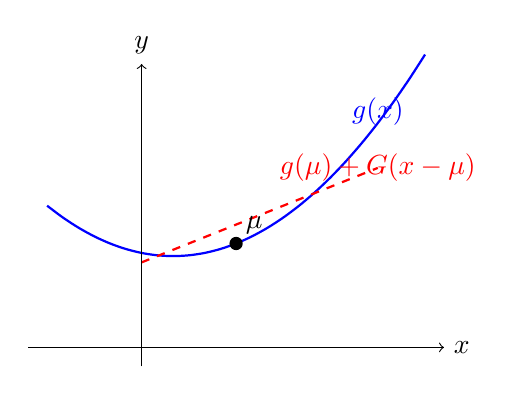
\begin{tikzpicture}[scale=1.2]
    % Nonlinear curve
    \draw[thick, blue] plot[smooth, domain=-1:3] (\x, {0.3*\x*\x - 0.2*\x + 1});

    % Tangent line
    \draw[thick, red, dashed] plot[domain=0:2.5] (\x, {0.4*\x + 0.9});

    % Point of linearization
    \fill (1, 1.1) circle (2pt) node[above right] {$\mu$};

    % Labels
    \node[blue] at (2.5, 2.5) {$g(x)$};
    \node[red] at (2.5, 1.9) {$g(\mu) + G(x-\mu)$};

    % Axes
    \draw[->] (-1.2,0) -- (3.2,0) node[right] {$x$};
    \draw[->] (0,-0.2) -- (0,3) node[above] {$y$};
\end{tikzpicture}
\caption{EKF linearizes nonlinear function around current estimate}
\end{figure}

\subsubsection{The Extended Kalman Filter Algorithm}

\begin{algorithm}[H]
\caption{Extended Kalman Filter}
\KwInput{$\mu_{t-1}$, $\Sigma_{t-1}$, $u_t$, $z_t$}
\KwOutput{$\mu_{t}$, $\Sigma_{t}$}

\BlankLine
\tcp{Compute Jacobian of dynamics}
$G_t = \frac{\partial g}{\partial x}\bigg|_{x=\mu_{t-1}, u=u_t}$\;

\BlankLine
\tcp{Prediction Step}
$\bar{\mu}_t = g(\mu_{t-1}, u_t)$\;
$\bar{\Sigma}_t = G_t \Sigma_{t-1} G_t^T + R_t$\;

\BlankLine
\tcp{Compute Jacobian of measurement model}
$H_t = \frac{\partial h}{\partial x}\bigg|_{x=\bar{\mu}_t}$\;

\BlankLine
\tcp{Kalman Gain}
$K_t = \bar{\Sigma}_t H_t^T (H_t \bar{\Sigma}_t H_t^T + Q_t)^{-1}$\;

\BlankLine
\tcp{Measurement Update}
$\mu_t = \bar{\mu}_t + K_t (z_t - h(\bar{\mu}_t))$\;
$\Sigma_t = (I - K_t H_t)\bar{\Sigma}_t$\;

\BlankLine
\Return{$\mu_{t}$, $\Sigma_{t}$}
\end{algorithm}

\textbf{Differences from KF:}
\begin{enumerate}
    \item Use $g(\mu_{t-1}, u_t)$ instead of $A\mu_{t-1} + Bu_t$
    \item Use $h(\bar{\mu}_t)$ instead of $C\bar{\mu}_t$
    \item Use Jacobians $G_t, H_t$ instead of constant matrices $A, C$
    \item Jacobians must be recomputed each timestep at current estimate
\end{enumerate}

\subsubsection{When Does EKF Work Well?}

\textbf{EKF approximation quality depends on:}

\begin{enumerate}
\item \textbf{Degree of nonlinearity:}
\begin{itemize}
    \item Small nonlinearity $\Rightarrow$ linear approximation good
    \item High nonlinearity $\Rightarrow$ approximation degrades
\end{itemize}

\item \textbf{Uncertainty magnitude:}
\begin{itemize}
    \item Small $\Sigma$ $\Rightarrow$ stay near linearization point $\Rightarrow$ good
    \item Large $\Sigma$ $\Rightarrow$ venture far from linearization point $\Rightarrow$ poor
\end{itemize}
\end{enumerate}

\textbf{Failure modes:}
\begin{itemize}
    \item Highly nonlinear systems with large uncertainty
    \item Linearization point far from true state
    \item Can lead to divergence or inconsistent estimates
\end{itemize}

% ============================================================================
\subsection{Unscented Kalman Filter (UKF)}
% ============================================================================

\subsubsection{Motivation}

\textbf{Problem with EKF:} Linearization can introduce significant errors, especially for highly nonlinear systems.

\textbf{UKF Key Idea:} Instead of linearizing functions, deterministically sample points (sigma points) around the mean, propagate them through the nonlinear function, then compute statistics.

\textbf{Philosophy:} "It's easier to approximate a probability distribution than to approximate an arbitrary nonlinear function."

\subsubsection{The Unscented Transform}

For state dimension $n$, generate $2n+1$ \textbf{sigma points}:
\begin{align}
\mathcal{X}^{[0]} &= \mu \\
\mathcal{X}^{[i]} &= \mu + \left(\sqrt{(n+\lambda)\Sigma}\right)_i, \quad i = 1, \ldots, n \\
\mathcal{X}^{[i]} &= \mu - \left(\sqrt{(n+\lambda)\Sigma}\right)_{i-n}, \quad i = n+1, \ldots, 2n
\end{align}

where $\lambda = \alpha^2(n + \kappa) - n$ is a scaling parameter and $\left(\sqrt{\Sigma}\right)_i$ is the $i$-th column of the matrix square root.

\textbf{Weights:}
\begin{align}
w_m^{[0]} &= \frac{\lambda}{n + \lambda} \\
w_c^{[0]} &= \frac{\lambda}{n + \lambda} + (1 - \alpha^2 + \beta) \\
w_m^{[i]} = w_c^{[i]} &= \frac{1}{2(n + \lambda)}, \quad i = 1, \ldots, 2n
\end{align}

Typical values: $\alpha = 10^{-3}$, $\beta = 2$ (optimal for Gaussian), $\kappa = 0$ or $3-n$.

\subsubsection{UKF Algorithm}

\begin{algorithm}[H]
\caption{Unscented Kalman Filter}
\KwInput{$\mu_{t-1}$, $\Sigma_{t-1}$, $u_t$, $z_t$}
\KwOutput{$\mu_{t}$, $\Sigma_{t}$}

\BlankLine
\tcp{Generate sigma points}
$\lambda = \alpha^2(n+\kappa) - n$\;
$\mathcal{X}_{t-1} = [\mu_{t-1} \quad \mu_{t-1} + \gamma\sqrt{\Sigma_{t-1}} \quad \mu_{t-1} - \gamma\sqrt{\Sigma_{t-1}}]$ where $\gamma = \sqrt{n + \lambda}$\;

\BlankLine
\tcp{Prediction: Propagate sigma points through dynamics}
\For{$i = 0$ to $2n$}{
    $\mathcal{X}_{t|t-1}^{[i]} = g(\mathcal{X}_{t-1}^{[i]}, u_t)$\;
}

\BlankLine
\tcp{Predict mean and covariance}
$\bar{\mu}_t = \sum_{i=0}^{2n} w_m^{[i]} \mathcal{X}_{t|t-1}^{[i]}$\;
$\bar{\Sigma}_t = \sum_{i=0}^{2n} w_c^{[i]} (\mathcal{X}_{t|t-1}^{[i]} - \bar{\mu}_t)(\mathcal{X}_{t|t-1}^{[i]} - \bar{\mu}_t)^T + R_t$\;

\BlankLine
\tcp{Regenerate sigma points from prediction}
$\bar{\mathcal{X}}_t = [\bar{\mu}_t \quad \bar{\mu}_t + \gamma\sqrt{\bar{\Sigma}_t} \quad \bar{\mu}_t - \gamma\sqrt{\bar{\Sigma}_t}]$\;

\BlankLine
\tcp{Propagate through measurement model}
\For{$i = 0$ to $2n$}{
    $\mathcal{Z}_t^{[i]} = h(\bar{\mathcal{X}}_t^{[i]})$\;
}

\BlankLine
\tcp{Predicted measurement statistics}
$\hat{z}_t = \sum_{i=0}^{2n} w_m^{[i]} \mathcal{Z}_t^{[i]}$\;
$S_t = \sum_{i=0}^{2n} w_c^{[i]} (\mathcal{Z}_t^{[i]} - \hat{z}_t)(\mathcal{Z}_t^{[i]} - \hat{z}_t)^T + Q_t$\;
$\bar{\Sigma}_t^{x,z} = \sum_{i=0}^{2n} w_c^{[i]} (\bar{\mathcal{X}}_t^{[i]} - \bar{\mu}_t)(\mathcal{Z}_t^{[i]} - \hat{z}_t)^T$\;

\BlankLine
\tcp{Kalman gain and update}
$K_t = \bar{\Sigma}_t^{x,z} S_t^{-1}$\;
$\mu_t = \bar{\mu}_t + K_t(z_t - \hat{z}_t)$\;
$\Sigma_t = \bar{\Sigma}_t - K_t S_t K_t^T$\;

\BlankLine
\Return{$\mu_{t}$, $\Sigma_{t}$}
\end{algorithm}

\subsubsection{UKF vs EKF}

\begin{tabular}{|l|l|l|}
\hline
\textbf{Property} & \textbf{EKF} & \textbf{UKF} \\
\hline
Jacobian computation & Required & Not needed \\
Accuracy (nonlinear) & First-order approx. & Second-order approx. \\
Computational cost & Lower & Moderate \\
Implementation & Simpler & More complex \\
Divergence risk & Higher & Lower \\
\hline
\end{tabular}

\vspace{3mm}
\textbf{When to use UKF:}
\begin{itemize}
    \item High nonlinearity
    \item Difficult to compute Jacobians
    \item Better accuracy needed
    \item Distribution approximately Gaussian
\end{itemize}

% ============================================================================
\section{Exam Tips \& Common Mistakes}
% ============================================================================

\begin{tcolorbox}[colback=red!10!white,colframe=red!75!black,title=\textbf{Common Exam Mistakes}]

\textbf{1. Jacobian Indexing:}
\begin{itemize}
    \item Remember: row = output equation, column = state variable
    \item Double-check dimensions: $G$ should be $n \times n$ for $n$ states
\end{itemize}

\textbf{2. Evaluation Point:}
\begin{itemize}
    \item $G_t$ evaluated at $\mu_{t-1}$ (before prediction)
    \item $H_t$ evaluated at $\bar{\mu}_t$ (after prediction)
\end{itemize}

\textbf{3. Discretization:}
\begin{itemize}
    \item Don't forget $\Delta t$ when discretizing!
    \item Euler: $x_t = x_{t-1} + \dot{x}_{t-1} \Delta t$
\end{itemize}

\textbf{4. Process Noise Location:}
\begin{itemize}
    \item $R_t$ adds to predicted covariance: $\bar{\Sigma}_t = G\Sigma G^T + R_t$
    \item $Q_t$ adds in Kalman gain: $(H\bar{\Sigma}H^T + Q_t)^{-1}$
\end{itemize}

\textbf{5. Innovation:}
\begin{itemize}
    \item $(z_t - h(\bar{\mu}_t))$ not $(z_t - \bar{\mu}_t)$
    \item Must pass prediction through measurement model!
\end{itemize}

\end{tcolorbox}

% ============================================================================
% END OF KALMAN FILTER NOTES
% ============================================================================
